
\documentclass{article}
\usepackage{url,graphicx,tabularx,array,geometry, hyperref}
\usepackage{listings}
\usepackage{fullpage}
\usepackage{fancyvrb}
\usepackage{framed}
\usepackage{lastpage}
\usepackage{fancyhdr}
\usepackage{float}

\renewcommand{\headrulewidth}{0pt}
\setcounter{secnumdepth}{0}

\setlength{\parskip}{1ex} %--skip lines between paragraphs
\setlength{\parindent}{0pt} %--don't indent paragraphs
\setlength{\headheight}{15.2pt}

\pagestyle{fancy}

\renewcommand{\headrulewidth}{0pt}
\lhead{  }
\lfoot{Lab 1: TCP Congestion Control}
\rfoot{page \thepage\ of \pageref{LastPage}}

\renewcommand{\familydefault}{\sfdefault}
\begin{document}

\begin{titlepage}
\begin{center}
\textsc{\huge \bfseries Advanced Networking 2018}\\[1.5cm]
\textsc{\large Lab \#1: TCP Congestion Control}\\[1.5cm]
\textsc{\huge Report}\\[1.5cm]
\textsc{\huge \bfseries GROUP: 3}\\[1.5cm]
\textsc{\large{\textbf{Authors:}\\ 
Kotaiba Alachkar, Kotaiba.Alachkar@os3.nl\\ Andrey Afanas'yev, Andrey.Afanasyev@os3.nl\\
Rick van Gorp, Rick.Vangorp@os3.nl\\
Henri Trenquier, Henri.Trenquier@os3.nl
}}

\textsc{\large University of Amsterdam}
\end{center}
\end{titlepage}
\subsection{Q0.0 Preparation}

\textsc{\large Configuration of the switch:}

We used \textit{Calais} to connect to the \textit{Mgmt} network.
From there, we configured \textit{Calais} to connect the Switch \textit{Chico3}:

\begin{verbatim}
    ## AN lab2 ##
auto eno2
iface eno2 inet static
        address 10.0.1.203 #mgmt
        netmask 255.255.255.0
        broadcast 255.255.255.255
\end{verbatim}

After restarting the network service, we can connect to \textit{10.0.1.4} via ssh.
From the switch, we can access the second port with
\begin{verbatim}
    dialout@serialserv4:~ $ minicom -b 9600 -D /dev/ttyUSB1
\end{verbatim}

We can now configure the switch:
\begin{verbatim}
 !
 no service password-encryption
 !
 ip domain-name gr3.com
 !
 hostname gr3switch
 !
 interface Vlan1
 ip address 192.168.0.253 255.255.255.0
 !
 interface Loopback1
 no ip address
 !
 username andrey password 0 cisco
 username kotaiba password 0 cisco
 username rick password 0 cisco
 username henrilarose password 0 cisco
 !
 line con 0
 logging synchronous
 login local
line vty 0 4
 password 7cisco
 login local
 transport input ssh
line vty 5 15
 login
 !
\end{verbatim}

\textsc{\large Connection to the network:}

Later, we can disconnect the UTP connection to the \textit{Mgmt} and connect to \textit{gr3switch}.

The new interface configuration is:
\begin{verbatim}
    ## AN lab2 ##
auto eno2
iface eno2 inet static
        address 192.168.0.127
        netmask 255.255.255.0
        broadcast 255.255.255.255
\end{verbatim}

If we encounter this error:
\begin{verbatim}
    RTNETLINK answers: File exists 
    Failed to bring up eno2
\end{verbatim}

The following command has to be entered:
\begin{verbatim}
    sudo ip addr flush dev eno2
\end{verbatim}

Finally, it is possible to connect to the local network. We can ping every team member from Henri's server.:
Ping Rick:
\begin{verbatim}
    ~ \$ ping 192.168.0.200
PING 192.168.0.200 (192.168.0.200) 56(84) bytes of data.
64 bytes from 192.168.0.200: icmp_seq=1 ttl=64 time=0.391 ms
64 bytes from 192.168.0.200: icmp_seq=2 ttl=64 time=0.181 ms
^C
--- 192.168.0.200 ping statistics ---
2 packets transmitted, 2 received, 0% packet loss, time 999ms
rtt min/avg/max/mdev = 0.181/0.286/0.391/0.105 ms
\end{verbatim}
Ping Kotaiba:
\begin{verbatim}
    ~ \$ ping 192.168.0.69
PING 192.168.0.69 (192.168.0.69) 56(84) bytes of data.
64 bytes from 192.168.0.69: icmp_seq=1 ttl=64 time=0.295 ms
64 bytes from 192.168.0.69: icmp_seq=2 ttl=64 time=0.150 ms
^C
--- 192.168.0.69 ping statistics ---
2 packets transmitted, 2 received, 0% packet loss, time 999ms
rtt min/avg/max/mdev = 0.150/0.222/0.295/0.074 ms
\end{verbatim}
Ping Andrey:
\begin{verbatim}
    ~ \$ ping 192.168.0.3
PING 192.168.0.3 (192.168.0.3) 56(84) bytes of data.
64 bytes from 192.168.0.3: icmp_seq=1 ttl=64 time=0.205 ms
64 bytes from 192.168.0.3: icmp_seq=2 ttl=64 time=0.083 ms
^C
--- 192.168.0.3 ping statistics ---
2 packets transmitted, 2 received, 0% packet loss, time 999ms
rtt min/avg/max/mdev = 0.083/0.144/0.205/0.061 ms
\end{verbatim}
Ping the switch:
\begin{verbatim}
    ~ \$ ping 192.168.0.253
PING 192.168.0.253 (192.168.0.253) 56(84) bytes of data.
64 bytes from 192.168.0.253: icmp_seq=2 ttl=255 time=1.78 ms
^C
--- 192.168.0.253 ping statistics ---
2 packets transmitted, 1 received, 50% packet loss, time 999ms
rtt min/avg/max/mdev = 1.783/1.783/1.783/0.000 ms
\end{verbatim}


Finally, we can connect via ssh with the following command:
\begin{verbatim}
~ \$ ssh -o KexAlgorithms=diffie-hellman-group1-sha1  henri@192.168.0.253    
\end{verbatim}

Indeed, the switch's configuration doesn't allow more recent Key exchange algorithm.

To disable HTTP and HTTPS we use the following commands:
\begin{verbatim}
gr3switch(config)#no ip http server
gr3switch(config)#no ip http secure-server
\end{verbatim}


To disable Telnet on other Virtual Terminal lines:
\begin{verbatim}
gr3switch(config)#line vty 5 15
gr3switch(config-line)#transport input none
\end{verbatim}

\subsection{Q2.1 Data transfer without and with CoS configuration}
In this question we have used \textit{iperf} to transfer data between 192.168.0.69 and 192.168.0.200. The server has been set up using \texttt{iperf -s} and the client connected to the server using \texttt{iperf -c -u 192.168.0.69} and \texttt{iperf -c 192.168.0.69}. We have not selected a specific congestion algorithm as the switch is a Gigabit-switch, which matches the speed of the NICs of the servers. The throughput achieved is listed in \textit{Figure \ref{fig:throughput_iperf}} and \textit{Figure \ref{fig:throughput_iperf2}}. We have also tested using different requested window sizes: 100, 100.000 and 100.000.000 bytes. This did not improve the speed, compared to \texttt{iperf's} defaults.

\bigskip

\begin{figure}[h]
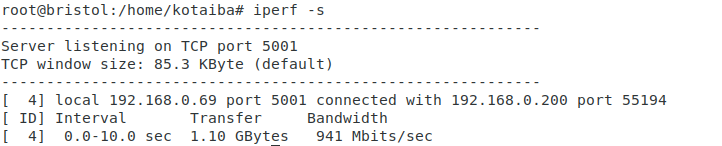
\includegraphics[width=8cm]{figures/q2-1-1.png}
\centering
\caption{TCP Performance}
\centering
\label{fig:throughput_iperf}
\end{figure}



\bigskip

\begin{figure}[h]
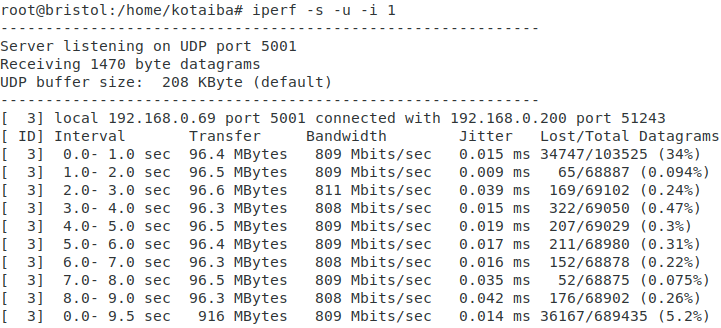
\includegraphics[width=8cm]{figures/q2-1-2.png}
\centering
\caption{UDP Performance}
\centering
\label{fig:throughput_iperf2}
\end{figure}


However, when we change the size of the MTU on interface \texttt{eno2}, the throughput increases.
%Todo: Do the experiment on higher MTU

\bigskip

\subsection{Q2.2 Define a number of scenarios where the data transfers interfere with each other}
After some discussion we could define following scenarios:

\begin{enumerate}
    \item Example from lab one basic scenario could be the one in which multiple nodes and applications are trying to  communicate  with  one  node.
        \begin{itemize}
            \item Server node required to run two \textit{iperf} servers accepting the TCP and UDP traffic. Other two nodes generates TCP and UDP traffic respectively.
        \end{itemize}
    \item A single node communicates with another node while the rest two try to ping first host at higher time frequency and with large packet sizes (DDOS).
        \begin{itemize}
            \item Two nodes communicate using iperf running on TCP (server and client).
            \item The rest two have a ping a iperf server with the same ping configuration like: \texttt{ping -i 0.01 -s 65507 192.168.0.200}
        \end{itemize}    
    \item One node has a HTTP/1.1 server on board which stress tested by other two nodes another node communicates with first one via \texttt{iperf}.
    \begin{itemize}
        \item One server is configured with Nginx and HTTP/1.1 it has also iperf server on board
        \item Two nodes try to stress test Nginx using simple ab test like \textitt{ab -n 1000000 -c 100 http://192.168.0.200/}
        \item Last one node is an iperf client.
    \end{itemize}
\end{enumerate}

\subsubsection{Execution of the first scenario}
We have set up the first scenario by setting up two \texttt{iperf} listeners (UDP and TCP) on server \texttt{192.168.0.200}, using commands \texttt{iperf -s} for TCP and \texttt{iperf -s -p 5000 -u} for UDP. The clients then connected to the server's listeners using commands \texttt{iperf -c 192.168.0.200} and \texttt{iperf -c 192.168.0.200 -p 5000 -u -b 1200M}. The results of this test are shown in \textit{Figure \ref{fig:scenario1_result1}} and \textit{Figure \ref{fig:scenario1_result2}}.

\begin{figure}[H]
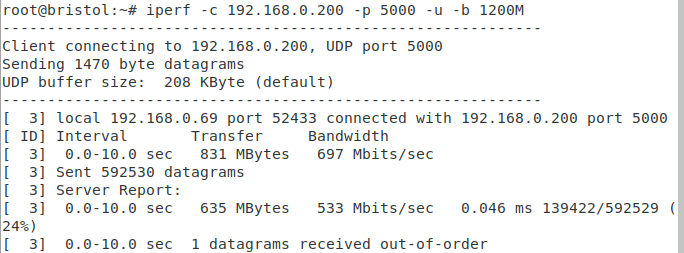
\includegraphics[width=14cm]{figures/q2-2-1-udp-1.png}
\centering
\caption{Scenario 1 - UDP Test 1}
\centering
\label{fig:throughput_udp_test_1}
\end{figure}


\begin{figure}[H]
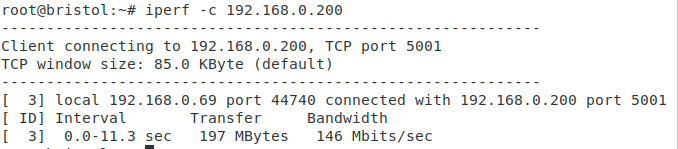
\includegraphics[width=14cm]{figures/q2-2-1-tcp-1.png}
\centering
\caption{Scenario 1 - TCP Test 1}
\centering
\label{fig:throughput_tcp_test_1}
\end{figure}


\begin{figure}[H]
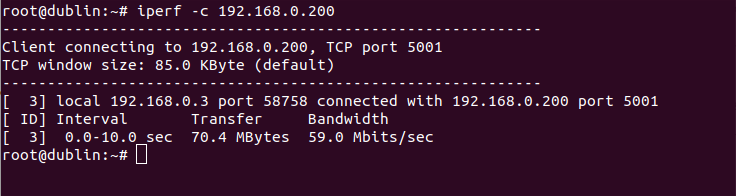
\includegraphics[width=14cm]{figures/q2-2-1-udp-2.png}
\centering
\caption{Scenario 1 - UDP Test 2}
\centering
\label{fig:throughput_udp_test_2}
\end{figure}


\begin{figure}[H]
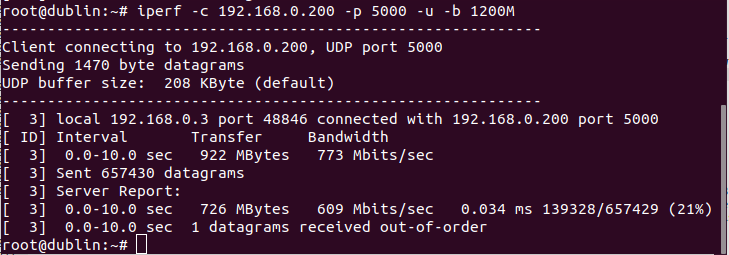
\includegraphics[width=14cm]{figures/q2-2-1-tcp-2.png}
\centering
\caption{Scenario 1 - TCP Test 2}
\centering
\label{fig:throughput_tcp_test_2}
\end{figure}


\begin{figure}[H]
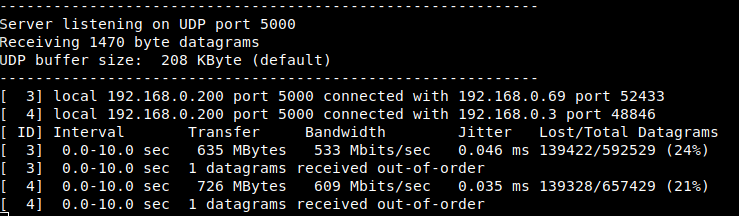
\includegraphics[width=14cm]{figures/q2-2-1-udp-result.png}
\centering
\caption{Scenario 1 - UDP Test result}
\centering
\label{fig:throughput_udp_result}
\end{figure}


\begin{figure}[H]
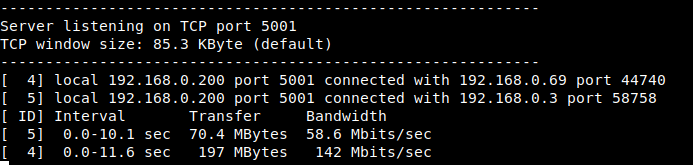
\includegraphics[width=14cm]{figures/q2-2-1-tcp-result.png}
\centering
\caption{Scenario 1 - TCP Test result}
\centering
\label{fig:throughput_tcp_result}
\end{figure}



\subsubsection{Execution of the second scenario}
In the second scenario we have set up an \texttt{iperf} server on \texttt{192.168.0.200}. We started a transfer on TCP towards the server in \texttt{iperf} from one client using \texttt{iperf -c 192.168.0.200}. At the same time, another pair of clients start a ping with large packet sizes using command \texttt{ping 192.168.0.200 -i 0.01 -s 65507}. The results are listed in \textit{Figure..}.






\begin{figure}[H]
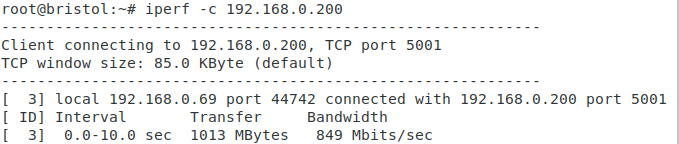
\includegraphics[width=14cm]{figures/q2-2-2-1.png}
\centering
\caption{Scenario 2 - TCP Iperf}
\centering
\label{fig:throughput_scenario_2}
\end{figure}

\begin{figure}[H]
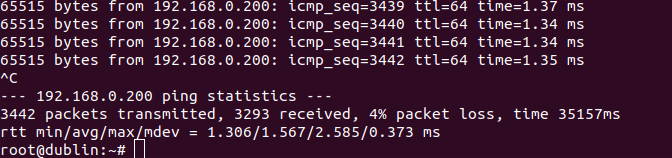
\includegraphics[width=14cm]{figures/q2-2-2-ping-2.png}
\centering
\caption{Scenario 2 - Large packet 1}
\centering
\label{fig:throughput_scenario_2_ping_1}
\end{figure}

\begin{figure}[H]
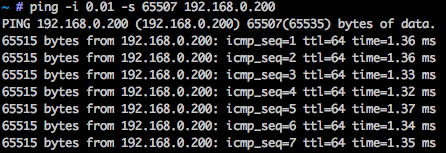
\includegraphics[width=14cm]{figures/q2-2-2-ping-1.png}
\centering
\caption{Scenario 2 - Large packet 2}
\centering
\label{fig:throughput_scenario_2_ping_2}
\end{figure}


\begin{figure}[H]
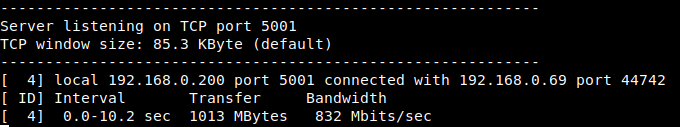
\includegraphics[width=14cm]{figures/q2-2-2-result.png}
\centering
\caption{Scenario 2 - Result}
\centering
\label{fig:throughput_scenario_2_result}
\end{figure}




\subsubsection{Execution of the third scenario}
In the third scenario will include an \texttt{Apache} webserver along with an \texttt{iperf} server running on \texttt{192.168.0.200}. One client will communicate with the server using \texttt{iperf -c 192.168.0.200} and the other two nodes will use a benchmarking tool like apache benchmark (ab) with the following command \texttt{b -n 100000 -c 10 http://192.168.0.200}


\begin{figure}[H]
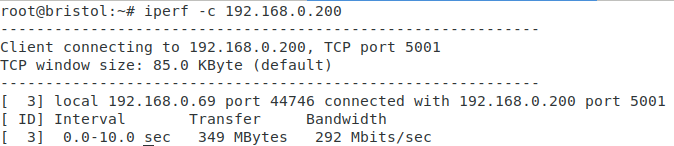
\includegraphics[width=14cm]{figures/q-2-2-3-1.png}
\centering
\caption{Scenario 2 - TCP Iperf}
\centering
\label{fig:throughput_scenario_3}
\end{figure}


\begin{figure}[H]
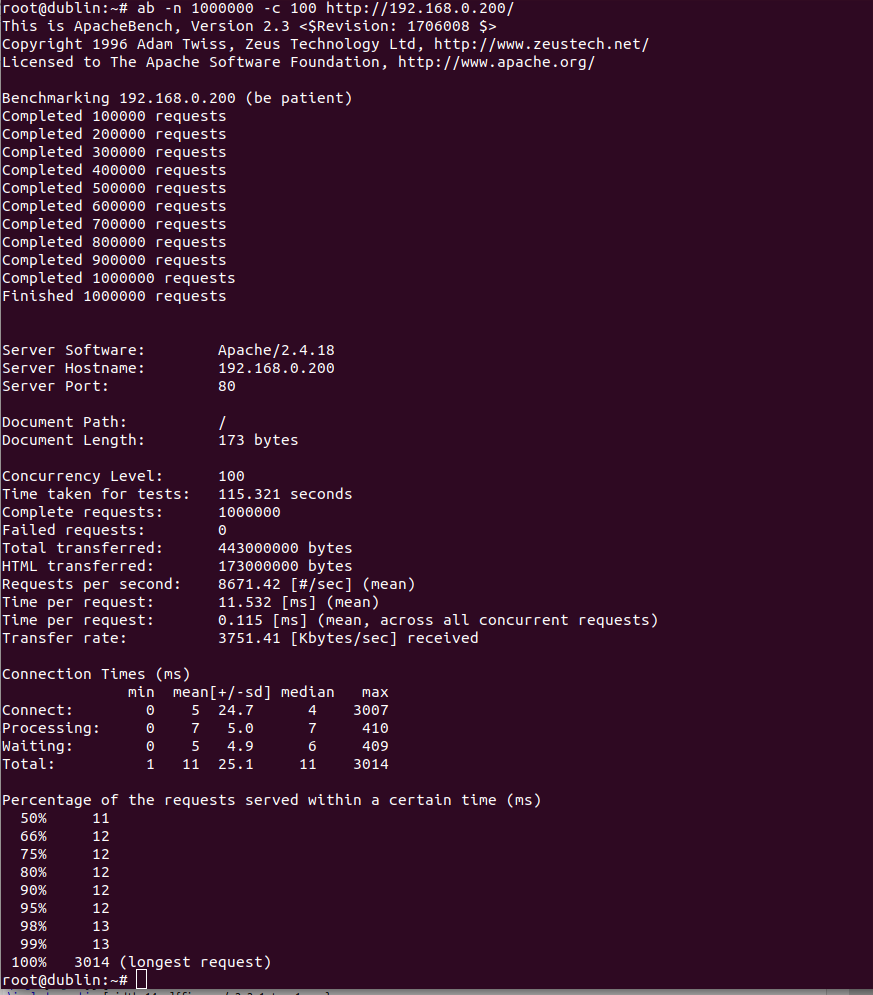
\includegraphics[width=14cm]{figures/dublin-ab.png}
\centering
\caption{Scenario 3 - Apache Benchmark from Dublin client server to Apache server}
\centering
\label{fig:ab_dublin_scenario_3}
\end{figure}

\begin{figure}[H]
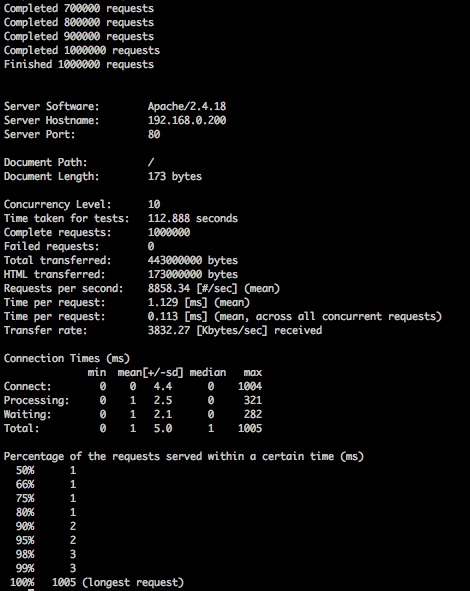
\includegraphics[width=14cm]{figures/calais-ab.png}
\centering
\caption{Scenario 3 - Apache Benchmark from client server to Apache server}
\centering
\label{fig:ab_calais_scenario_3}
\end{figure}




\begin{figure}[H]
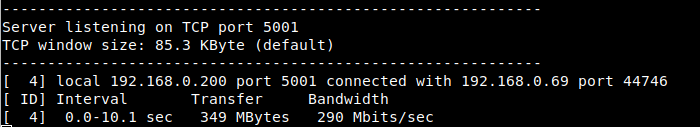
\includegraphics[width=14cm]{figures/q-2-2-3-results.png}
\centering
\caption{Scenario 2 - Result}
\centering
\label{fig:throughput_scenario_3_result}
\end{figure}


\subsection{Q3 Configuring CoS}
In order to configure CoS, it has to be enabled on the interfaces of the switch where the servers are connected to.

%Todo: Add description

\begin{figure}[H]
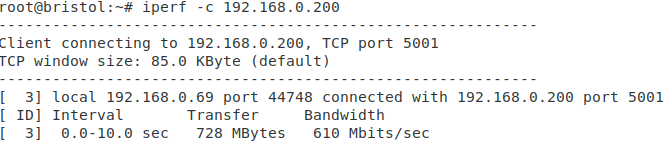
\includegraphics[width=14cm]{figures/q3-1-1.png}
\centering
\caption{Cos - TCP Iperf}
\centering
\label{fig:throughput_scenario_3}
\end{figure}


\begin{figure}[H]
\centering
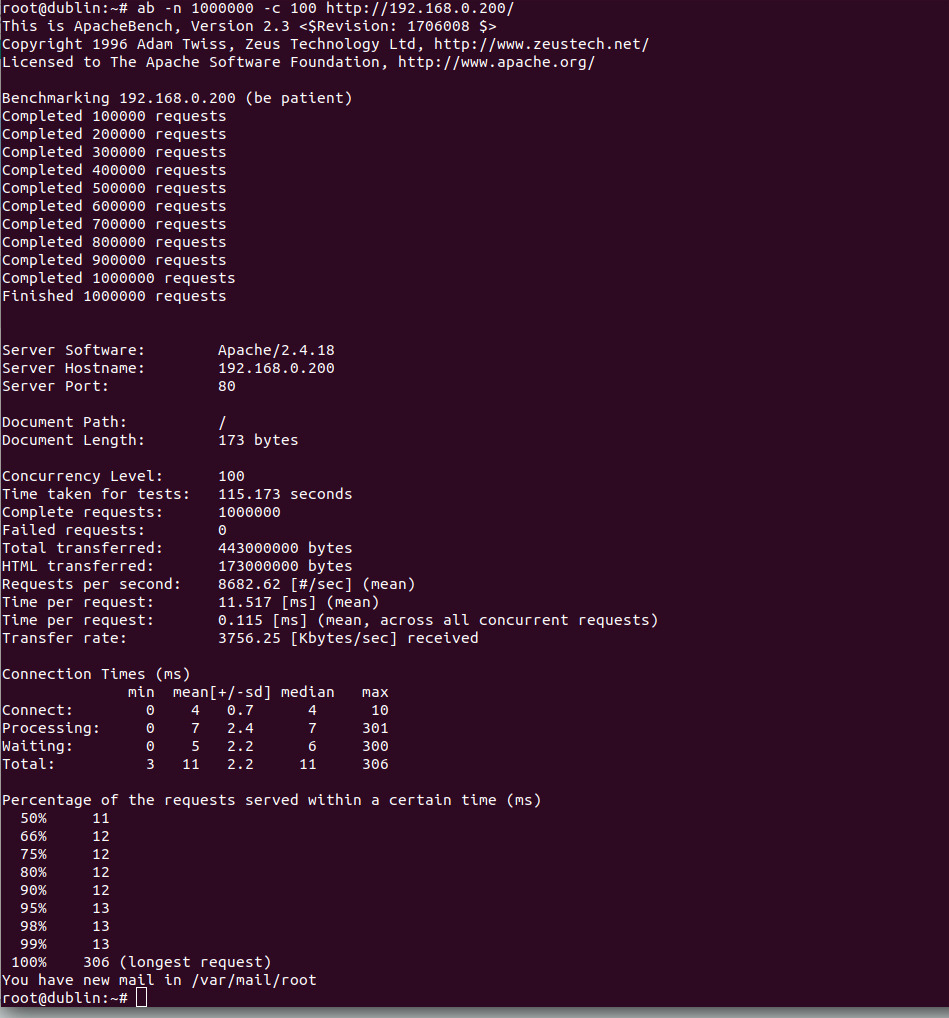
\includegraphics[width=14cm]{figures/dublin-ab2.png}
\caption{Cos - Apache Benchmark from Dublin client to Apache server with CoS enabled}
\centering
\label{fig:ab2_calais_scenario_3}
\end{figure}


\begin{figure}[H]
\centering
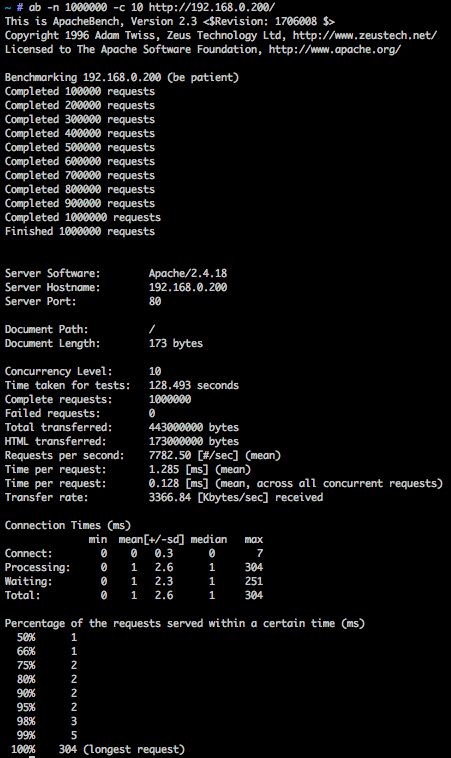
\includegraphics[width=12cm]{figures/calais-ab2.png}
\caption{Cos - Apache Benchmark from client to Apache server with CoS enabled}
\centering
\label{fig:ab2_calais_scenario_3}
\end{figure}

\subsubsection{Difference between SRR and other}

% Just going to put this here.
\begin{verbatim}
    gr3switch(config)#int G1/0/19
gr3switch(config-if)#no srr-
gr3switch(config-if)#no srr-queue bandwidth share 15 15 15 15
gr3switch(config-if)#int G1/0/17                             
gr3switch(config-if)#no srr-queue bandwidth share 15 15 15 15
gr3switch(config-if)#int G1/0/23
gr3switch(config-if)#no srr-queue
% Incomplete command.

gr3switch(config-if)#no srr-queue bandwidth
% Incomplete command.

gr3switch(config-if)#no srr-queue bandwidth share
gr3switch(config-if)#srr-queue bandwidth shape ?
  <0-65535>  enter bandwidth weight for queue id 1

gr3switch(config-if)#srr-queue bandwidth shape 45000 45000 45000 45000  
gr3switch(config-if)#int G1/0/19
gr3switch(config-if)#srr-queue bandwidth shape 9830 9830 9830 9830
gr3switch(config-if)#int G1/0/17
gr3switch(config-if)#srr-queue bandwidth shape 9830 9830 9830 9830

\end{verbatim}

\subsection{Q4.1 Mark your outgoing packets using iptables}
One of the characteristics of DSCP is that the classification of the packets can occur at the source (sender of specific traffic). The marking of the packets can be done using iptables, which is simply separating them into classes based on the protocol or ports used.\\
\\
Example rule (has to be fixed by actual rules, but depends on task 2):
%Todo: Make rules men ROGER THAT !!
\begin{verbatim}
iptables -t mangle -A OUTPUT -p udp -m udp --sport 5060 -j DSCP --set-dscp-class cs3
\end{verbatim}

\subsection{Q4.2 Show that the packets are marked}
In order to show the packets are marked, a \texttt{tcpdump} was started on one of the servers. The resulting PCAP-file was analysed using Wireshark. To check whether DSCP was applied to packets, we searched through the packets using filter \texttt{ip.dsfield.dscp}. The DSCP-value was retrieved from the \texttt{Differentiated Services Field} and ...
%TODO: CodePoint has to be shown, screenshot pls. Explain codepoint and relevance to IPTables rule.


\subsection{Q4.3 Show how DSCP marking improves traffic performance.}

% TODO: answer it LOL


\subsection{Q5.1 Enable logging of events (syslog) to an external server.}

By default, syslog is enabled in cisco switches by default. We just need to forward the log to our server. The following command will do that:

\begin{verbatim}
gr3switch(config)#logging host 192.168.0.69

Now inside /etc/rsyslog.conf 
# for cisco
local7.*        /var/log/cisco-messages.log
\end{verbatim}


\end{document}
